
\documentclass[12pt]{article}
\usepackage[a4paper,margin=1in]{geometry}
\usepackage[utf8]{inputenc}
\usepackage[T1]{fontenc}
\usepackage{amsmath,amssymb}
\usepackage{graphicx}
\graphicspath{{meta_images/}}
\usepackage{hyperref}
\usepackage{enumitem}
\usepackage{algorithm}
\usepackage{algorithmic}
\usepackage{booktabs}

% Editorial asides added during the 2026 digitization pass are wrapped in
% \editornote{...} so they're visually distinguishable from the 1997 text.
\newcommand{\editornote}[1]{\textit{[2026: #1]}}

\title{\textbf{Backpropagation Feed-Forward Neural Networks}}
\author{Vasili Gavrilov}
\date{Seminar in Artificial Intelligence (1997)}

\begin{document}
\maketitle

\begin{center}
  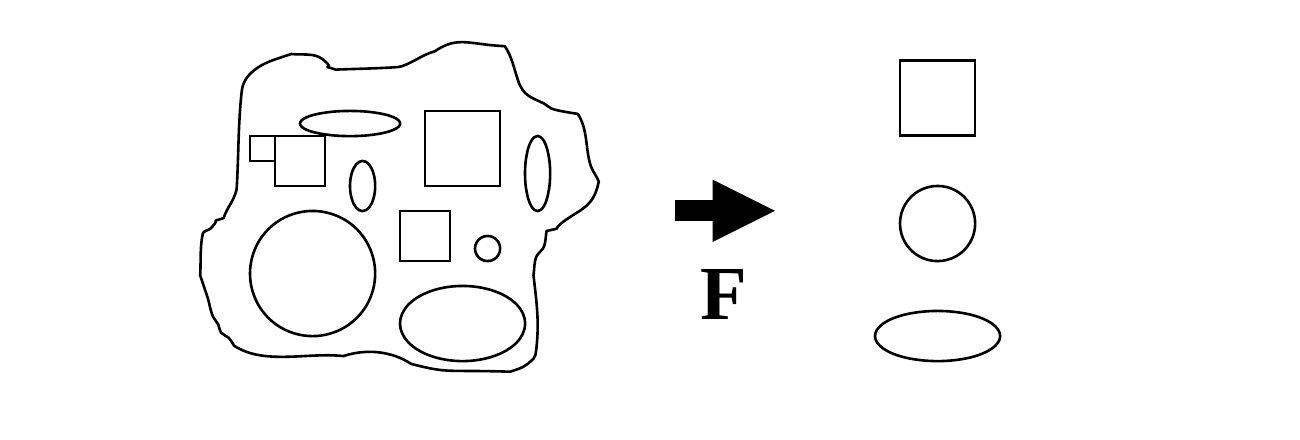
\includegraphics[width=0.55\textwidth]{pattern_classification.png}
\end{center}

\section*{Preface (2026)}

I wrote this in 1997 as a seminar thesis in neural networks, the work required to complete my undergraduate computer science degree. The task my professor gave me was to derive the delta-rule for multi-layer feed-forward networks in its general form: the prior work by Hinton and collaborators had established backpropagation at the perceptron level, and the seminar's job was to push the derivation through to the general multi-layer case. I worked it out in tensor form, and added a small meta-analysis of the existing NN literature of the time. In retrospect, amusing how few papers were available to survey. The illustrations are vintage MS Paint, drawn in a rush during the summer before I left for Canada.

For twenty-nine years it sat in a folder. The decision to publish came from an unexpected source: a long conversation with a large language model about a separate topic. At some point the model said the report might still be useful as a beginner's introduction to backpropagation feed-forward networks, because it is short, self-contained, math-first, builds from first principles, and old enough that nothing in it has the polish of a modern textbook.

That last bit is what made me pause. Most current tutorials assume you already know what a gradient is, drop you into PyTorch on page two, and treat backprop as a black box behind \texttt{loss.backward()}. This report does the opposite. It starts at the biological neuron, builds up the math, derives backpropagation from gradient descent and the chain rule, and ends with two real applications: cell classification for cancer diagnosis, and the LeCun handwritten-digit work that, in retrospect, is the origin story of convolutional networks.

For a beginner today the math is unchanged since 1986, and a reader with calculus (through partial derivatives) and basic linear algebra can follow the derivation cover-to-cover in one sitting. What is missing is mostly cosmetic: ReLU instead of sigmoid for activation, Adam instead of fixed-rate gradient descent, and the post-2012 deep-learning toolkit. None of that changes the foundations the report covers; you layer the modern material on top once the foundations are clear.

\begin{center}
\small\textit{Historical Note (2026). This document is a digitized archival release of a seminar coursework report originally completed in 1997 at the Open University of Israel under the supervision of Professor Ehud Gudes. The substance is preserved as a snapshot of early neural network methodology. Corrections and restorations made during the 2026 digitization pass: a few grammatical fixes; one tensor index aligned with the row-receives, column-sends convention used throughout; a weight-initialization range restored from a transcription error ($2.4\,f_i \rightarrow 2.4/f_i$); an author name order corrected (Ciamac Moallemi); the Rumelhart, Hinton, Williams 1986 backpropagation paper restored to the bibliography after being lost in transcription; several sections and fourteen of the original 1997 illustrations dropped by an earlier rewrite have been restored from the source PDF; and a duplicate ``meta-analysis'' applications section introduced by that rewrite has been removed. This is Ver.2 of the restoration: several additional pictures from the original that had been lost have since been found in the archive and reinserted.}
\end{center}

\newpage

\begin{abstract}
This coursework concerns backpropagation feed-forward neural networks (BPFFNNs), which historically comprised a large fraction of successful neural-network applications. The report reviews the main architectural ideas behind feed-forward networks, introduces the standard neuron model, and derives the generalized delta rule (backpropagation) as gradient descent in weight space, including a consistent tensor (matrix) form of the update. Two practical applications are discussed: classifying cells for cancer diagnosis and handwritten digit recognition. Finally, the report argues that incorporating problem-specific heuristics into the network topology and preprocessing is often necessary to obtain a network that is trainable, convergent, and able to generalize without severe underfitting or overfitting.
\end{abstract}

\tableofcontents
\newpage

\section{Introduction to Neural Networks}
In this report, \emph{neural networks} (NN) refers to \emph{artificial neural networks} (ANNs): mathematical models inspired by biological neural systems. Historically, the original goal of ANNs was to model and simulate biological neural computation. In modern usage, however, ``neural network'' is frequently used for engineered systems whose architecture and operation may differ substantially from biology.

Although there are many definitions, most share a common core: a neural network is a massively parallel, distributed processor (typically without an overall system clock) that can learn from examples and often exhibits some capability for generalization beyond the training data. A neural network contains many simple interconnected processing elements with local memory rather than a small number of complex processors. Each element operates primarily on local information and can operate asynchronously.

In a broad sense, neural networks can be viewed as a non--von Neumann approach to computation, where many competing hypotheses are processed simultaneously. Implementations range from software simulators to dedicated hardware accelerators.

\subsection{Differences from the von Neumann model}
In a von Neumann computer the programmer must know in advance the exact sequence of steps the algorithm performs. The advantage of NN is the absence of that requirement: it is sufficient to supply the network with enough well-chosen examples of the desired input--output behavior, which can be considered as ``teaching'' the network. Selecting a good training set may take more time and effort than the training itself. A NN cannot predict a non-existent function, but it can approximate any mapping between input and output spaces (any computable function) given enough resources and training data.

The main features distinguishing a NN from a traditional digital computer are:
\begin{itemize}[leftmargin=1.2em]
  \item Signal processing (rather than symbol processing).
  \item Information stored in weights (rather than in a program).
  \item Robustness in the presence of noise: small input perturbations do not collapse the output.
  \item Robustness to partial hardware failure: damage affects only a subset of outputs rather than disabling the system.
  \item High-level concepts distributed across the whole network rather than localized in one memory cell.
  \item Generalization: the ability to deal with patterns not seen during training.
\end{itemize}

NN are not more powerful in the formal sense than ordinary digital computers (they compute the same class of computable functions), but they make some tasks much easier than algorithmic programming does. Telling photographs of men from photographs of women, for instance, has no clean rule-based algorithm; yet a five-year-old performs it reliably, even when the woman has short hair. NN are well-suited to that kind of task.

\subsection{Comparison: brain vs.\ computer (1997 estimates)}
The biological inspiration is concrete in scale terms. \editornote{The orders-of-magnitude comparison below is roughly what the field reported in 1997; modern figures look very different.}

\begin{center}
\begin{tabular}{|l|c|c|}
\hline
                       & \textbf{Computer}        & \textbf{Brain}           \\
\hline
Computational units    & $10^5$ gates             & $10^{11}$ neurons        \\
Storage units          & $10^9$ RAM, $10^{10}$ disk & $10^{11}$ synapses     \\
Cycle time             & $10^{-8}$ seconds        & $10^{-3}$ seconds        \\
Bandwidth              & $10^9$ bits/sec          & $10^{14}$ bits/sec       \\
Neuron updates per sec & $10^5$                   & $10^{14}$                \\
\hline
\end{tabular}
\end{center}

An ANN simulator running on a von Neumann host needs roughly $10^2$ cycles to model a single neuron firing, while a brain performs all neuron updates simultaneously. The computer is about $10^6$ times faster at raw switching, yet a brain recognizes a face in under a second. The difference is massive parallelism. (Dedicated NN hardware or clusters narrow this gap; the comparison above assumes ANN simulated on a serial machine.) \editornote{This was already true in 1997 with the AT\&T ANNA chip and Connection Machines; it is overwhelmingly true today with GPUs.}

\subsection{Hardware perspective (Flynn's classification)}
Flynn's classification organizes computer architectures along two axes: how many instruction streams the machine executes at once, and how many data streams it operates on at once. The four resulting quadrants are:

\begin{center}
\begin{tabular}{|l|c|c|}
\hline
 & \textbf{Single Data Stream} & \textbf{Multiple Data Streams} \\
\hline
\textbf{Single Instruction Stream}
  & SISD                 & SIMD                  \\
  & (classical uniprocessor) & (vector / array processor) \\
\hline
\textbf{Multiple Instruction Streams}
  & MISD                 & MIMD                  \\
  & (rare; systolic array) & (multiprocessor, cluster) \\
\hline
\end{tabular}
\end{center}

Classical uniprocessors fall under SISD. Vector and array supercomputers (the Cray series, ILLIAC IV) are the canonical SIMD machines, applying one instruction to many data elements at once. Large multiprocessor systems and transputer-based hardware are MIMD. The MISD quadrant has few practical instances; systolic arrays are sometimes placed there.

Neural networks fit naturally into the MIMD model. Each neuron is conceptually an independent processor operating on its own inputs and weights. In practice, many neural computations (e.g., applying the same activation function across all units in a layer, or computing layer-wise vector--matrix products) are regular enough that SIMD hardware also accelerates them effectively; specialized chips for backpropagation networks of this period typically exploited that regularity.

\section{Neurons}

Since NN are based on the architecture of animal brains, we begin with a brief description of a real neuron. A neuron has many dendrites and (usually) one long axon; the axon contacts the dendrites of other cells through synapses. Treating the dendrites of a single cell as its inputs, the cell does nothing until the collective influence of all inputs (roughly $10^5$ per neuron) reaches the firing threshold. Knowledge is stored at the synapses as connection strengths (amounts of various chemical mediators), which we model as \emph{synaptic weights}. When the cell fires, a depolarization wave (a wave-like local Na$^+$/K$^+$ polarization) travels down the axon and reaches the synapses at its end, where it influences the next neuron in turn.

\begin{center}
  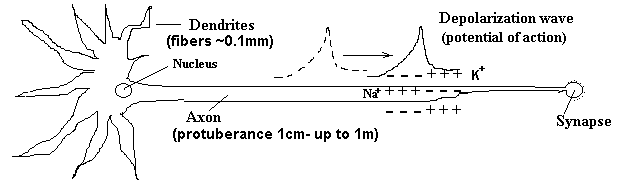
\includegraphics[width=0.78\textwidth]{neuron.png}
\end{center}

\subsection{The basic neuron model}
The computing units of an ANN are called \emph{artificial neurons}, or \emph{threshold logic units} (TLU). The basic schema is:

\begin{center}
  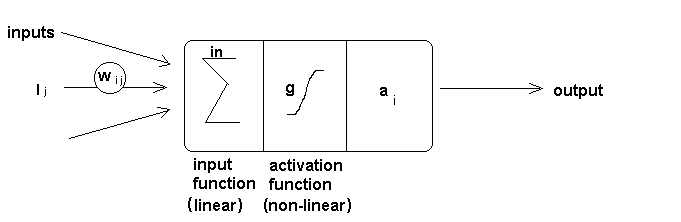
\includegraphics[width=0.72\textwidth]{perceptron.png}
\end{center}

Each incoming link carries an associated weight (a scalar parameter that determines how strongly one node influences another). A positive weight ($w>0$) is called an \emph{excitation}; a negative weight ($w<0$) is called an \emph{inhibition}. Weights are obtained from learning. For inputs $I_1,\dots,I_n$, weights $w_1,\dots,w_n$, and a threshold $\theta$, define the pre-activation
\begin{equation}
  \mathit{in}_i = \sum_{j=1}^{n} w_{ij} I_j,
\end{equation}
and the output
\begin{equation}
  a_i = g(\mathit{in}_i),
\end{equation}
where $g(\cdot)$ is the activation function. The neuron activates when $\mathit{in}_i$ reaches the threshold $\theta$; in vector form this condition is $\mathbf{w}\cdot\mathbf{I} \geq \theta$.

\subsection{Why nonlinearity is essential}
Note that $g$ cannot be linear; if it were, a multi-layer network would have the same expressive power as a single linear layer (since the sum of linear functions is linear). Nonlinear activation is therefore essential for representing non-linear decision boundaries and for approximating complex functions. Different methods may use different choices of $g$; the requirement is non-linearity. The three common choices are:

\begin{center}
\begin{tabular}{ccc}
\textbf{(a) Step function} & \textbf{(b) Sign function} & \textbf{(c) Sigmoid} \\
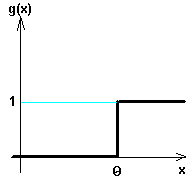
\includegraphics[width=0.22\textwidth]{activation_step.png} &
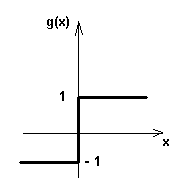
\includegraphics[width=0.22\textwidth]{activation_sign.png} &
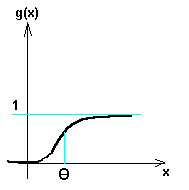
\includegraphics[width=0.22\textwidth]{activation_sigmoid.png} \\
$g(x) = \begin{cases} 1, & x \geq \theta \\ 0, & x < \theta \end{cases}$ &
$g(x) = \begin{cases} \phantom{-}1, & x \geq 0 \\ -1, & x < 0 \end{cases}$ &
$g(x) = \dfrac{1}{1+e^{-x}}$
\end{tabular}
\end{center}

The sigmoid is the most interesting choice for the purposes of this report: it is differentiable around the threshold $\theta$ (the chain rule below requires this). Other nonlinear functions also work in practice; an interesting example using $\sin(x)$ as activation is mentioned later. \editornote{Sigmoid was the 1997 default for hidden layers. Today the default is ReLU, $g(x)=\max(0,x)$, which removes the vanishing-gradient problem of deep sigmoid networks and trains much faster. Sigmoid is still used at output units for binary classification, and softmax for multi-class output.}

\subsection{Bias as an extra input}
A TLU with a separate threshold $\theta$ can be drawn as:

\begin{center}
  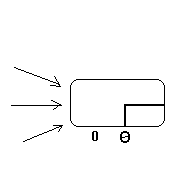
\includegraphics[width=0.22\textwidth]{ltu_basic.png}
\end{center}

It is often more convenient to fold the threshold into the weights themselves (so that learning adjusts weights only, not weights and a separate threshold) by introducing an extra input $I_0$:

\begin{center}
  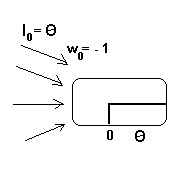
\includegraphics[width=0.30\textwidth]{ltu_bias_as_input.png}
\end{center}

\noindent With $I_{0i}=\theta$ and $w_{0i}=-1$, the threshold becomes
\begin{equation}
  w_{0i} I_{0i} = -\theta,
\end{equation}
and the activation condition collapses neatly:
\begin{equation}
  a_i = g(\mathit{in}_i) = g\!\left(\sum_{j=1}^n w_{ij} I_{ij}\right) = g\!\left(\sum_{j=0}^n w_{ij} I_{ij}\right).
\end{equation}

\subsection{Example: logic gates}
A single TLU with appropriate weights and a step activation implements any one of the basic Boolean functions. The classic three:

\begin{center}
  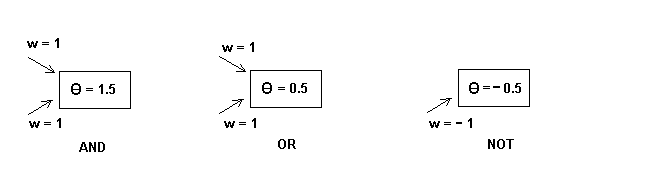
\includegraphics[width=0.75\textwidth]{logic_gates.png}
\end{center}

\noindent AND: $w_1=w_2=1$, $\theta=1.5$. OR: $w_1=w_2=1$, $\theta=0.5$. NOT: $w=-1$, $\theta=-0.5$. Since AND, OR, and NOT form a functionally complete set, any Boolean function can in principle be assembled from such elements.

\section{Feed-Forward Networks}
\subsection{Layered structure}
A feed-forward network is organized into layers: an input layer, one or more hidden layers, and an output layer. Information flows from inputs to outputs in a strictly feed-forward way. This is in contrast to recurrent networks, which contain feedback connections (Hopfield networks are a classical example).

\begin{center}
  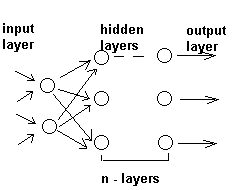
\includegraphics[width=0.45\textwidth]{ffnn_layers.png}
\end{center}

Let $a^{(\ell)}$ be the vector of activations in layer $\ell$. The feed-forward computation for layer $\ell$ is
\begin{align}
  z^{(\ell)} &= W^{(\ell)} a^{(\ell-1)} + b^{(\ell)},\\
  a^{(\ell)} &= g\!\left(z^{(\ell)}\right),
\end{align}
where $W^{(\ell)}$ is the weight matrix and $b^{(\ell)}$ is the bias vector.

The first studied network of this kind (1950s) was the \emph{perceptron}: a single-layer network with no hidden units. It is the most trivial network architecture. The limitations of perceptrons are revisited in the Learning section.

\begin{center}
  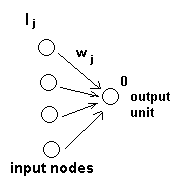
\includegraphics[width=0.28\textwidth]{single_perceptron_classifier.png}
\end{center}
\begin{center}
\small A single-layer perceptron: input nodes $I_j$ feed into one output unit through weights $w_j$, with no intermediate layer.
\end{center}

\subsection{Supervised and unsupervised learning}
A common distinction is between supervised and unsupervised learning networks. In supervised learning, an external ``teacher'' (supervisor) specifies the desired behavior during training. In unsupervised learning, the network self-organizes structure from the data (Kohonen networks are a standard example). Some networks do not learn at all (they compute a fixed function).

\subsection{Function approximation (informal)}
Feed-forward networks with at least one sufficiently large hidden layer can approximate a broad class of continuous functions on compact domains. In practice, approximation quality depends on the number of hidden units, the amount and quality of training data, and the effectiveness of the training algorithm.

There is no simple closed form for the ``ideal'' network architecture: network design is an art. The right architecture depends on the number of training cases, the noise level, and the complexity of the function being learned. Some problems with one input and one output need thousands of hidden units; some problems with thousands of inputs need almost none. In the sections that follow, all architectures are designed by hand rather than discovered automatically.

\section{Network Topology}
\subsection{Topology and inductive bias}
\emph{Network topology} is the pattern of connections among units. It determines how information propagates and encodes an \emph{inductive bias}: constraints that reduce the hypothesis space so learning is feasible with limited data.

In application work, topology is rarely chosen arbitrarily. It is usually adapted to the structure of the input domain (e.g., 2D geometry for images) and to invariances required for generalization (e.g., shift invariance in character recognition).

\section{Learning}

Learning (teaching, training) a network is the process of tuning its parameters to fit a training set. Many learning methods exist and new ones appear constantly; from a statistician's point of view a neural network performs nonlinear regression. The initial network has randomly assigned weights (zeros or small numbers close to zero). The network is updated to make it consistent with a sequence of input--output examples: small adjustments to weights reduce the difference between observed and predicted outputs. Updates are grouped into \emph{epochs} (one pass over all training examples). The process repeats until the error becomes negligibly small.

\subsection{Every node is a classifier}
Every node in the network behaves as a classifier, partitioning its input space into two regions. Consider a single perceptron node with two inputs (dropping the node index for clarity):

\begin{center}
  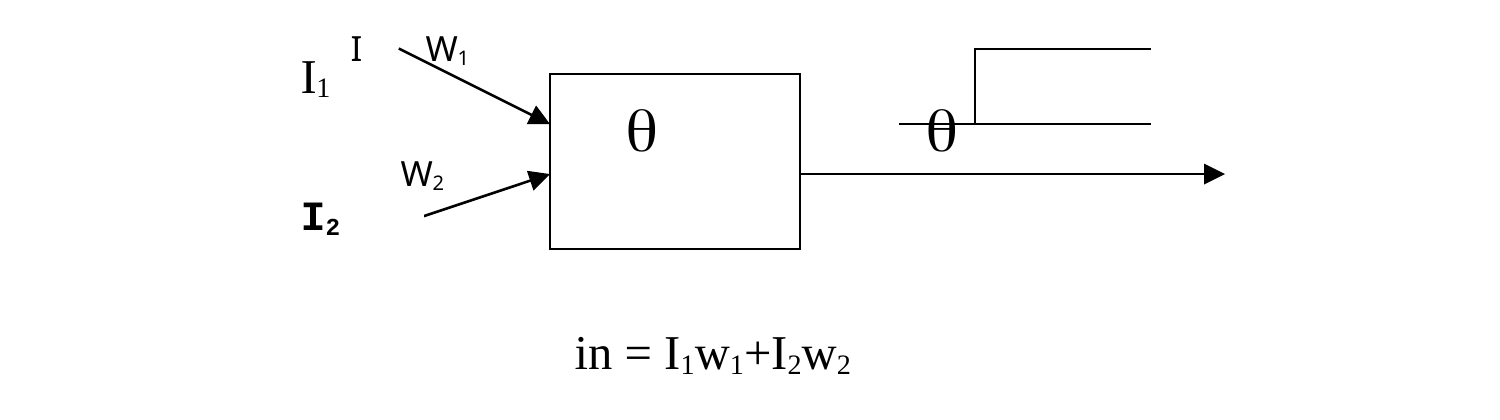
\includegraphics[width=0.55\textwidth]{perceptron_2d_classifier.png}
\end{center}
\begin{center}
\small Two-input perceptron with explicit inputs $I_1, I_2$, weights $w_1, w_2$, threshold $\theta$, and a step activation; the unit fires when the linear sum reaches $\theta$.
\end{center}

\noindent The activation condition $\mathbf{w}\cdot\mathbf{I} \geq \theta$ reads in components as
\begin{equation}
  w_1 I_1 + w_2 I_2 \geq \theta.
\end{equation}
Since this is a linear inequality, it corresponds to a half-plane in $(I_1, I_2)$ space separated by the line
\begin{equation}
  I_2 = -\frac{w_1}{w_2} I_1 + \frac{\theta}{w_2}.
\end{equation}
In general, with $n$ inputs the boundary is an $n$-dimensional hyperplane embedded in $(n+1)$-dimensional space.

\paragraph{Worked example.} Let $w_1 = w_2 = 1$ and $\theta = 1.5$. Substituting into $w_1 I_1 + w_2 I_2 = \theta$ gives $I_1 + I_2 = 1.5$. If inputs are restricted to $\{0,1\}$, the solutions partition the unit square:

\begin{center}
  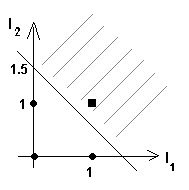
\includegraphics[width=0.25\textwidth]{linear_decision_boundary.png}
\end{center}

\noindent Learning the perceptron then reduces to adjusting $w$ and $\theta$ until the line separates the two classes.

\subsection{XOR and the limits of one perceptron}
Consider two regions in $(I_1, I_2)$ space where one is enclosed by the other; no single straight line separates them.

\begin{center}
  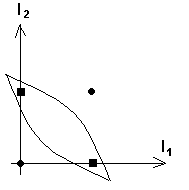
\includegraphics[width=0.25\textwidth]{xor_nonseparable.png}
\end{center}

\noindent The Boolean XOR function is the classical example of a linearly non-separable function. Rosenblatt's perceptron-convergence theorem (first proved in 1960) guarantees that the perceptron learning rule converges to a correct set of weights, provided the target function is linearly separable; in particular, a perceptron learns successfully only from noise-free, linearly-separable data. For functions like XOR the only remedy is to add a hidden unit:

\begin{center}
  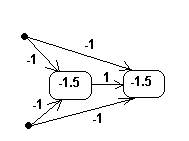
\includegraphics[width=0.30\textwidth]{xor_solved_2ltus.png}
\end{center}

\subsection{Training, test, and validation sets}
The standard terminology (following Ripley) is:

\begin{itemize}[leftmargin=1.2em]
  \item \textbf{Training set}: examples used for learning.
  \item \textbf{Test set}: examples used to evaluate performance.
  \item \textbf{Validation set}: examples used to tune classifier parameters (network topology, threshold function, etc.).
  \item \textbf{Generalization}: the property of the network to make correct predictions for cases that were not in the training set.
\end{itemize}

Consider the picture below: black dots are training examples, lighter ones are test examples. Even though the lighter dots were never used to fit the weights, they are still classified correctly: $A$ as $A$, $B$ as $B$.

\begin{center}
  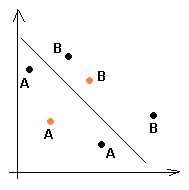
\includegraphics[width=0.28\textwidth]{ab_linearly_separable.png}
\end{center}

\noindent Generalization is the most critical issue in network design. In statistical terms it is the difference between interpolation (predicting within the range of training data) and extrapolation (predicting outside it). The main aim is to make the network rely on interpolation by collecting enough good training data, usually the hardest part of the project.

\subsection{Underfitting, overfitting, and the spline analogy}
A network that lacks enough internal degrees of freedom to model the target function will fail to fit even the training set. This is \emph{underfitting}: the network is too trivial, rigid, or low-capacity. The other extreme is \emph{overfitting}: the network has so many parameters that it can memorize the training data (including noise) without learning the underlying regularity.

A useful analogy is spline interpolation. To pass a curve through a set of pins, one could choose a flexible rope: it will pass through every pin perfectly, but the curve in between is essentially arbitrary and the rope has not learned anything generalizable about the data; it has memorized it. That is overfitting. At the opposite extreme, a stiff metal rod cannot bend enough to reach the pins at all; it captures only the simplest linear trend and misses everything else. That is underfitting. The ideal classifier is flexible enough to fit the data but rigid enough to derive the underlying knowledge rather than enumerate the inputs.

\begin{center}
  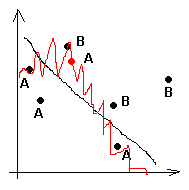
\includegraphics[width=0.28\textwidth]{ab_overfit_boundary.png}
\end{center}
\begin{center}
\small Overfitting and underfitting.
\end{center}

\noindent A practical rule of thumb is that the number of trainable weights influencing any output should be smaller than the number of training samples. Increasing the number of weights can speed convergence but increases the risk of overfitting; a very small network may not learn the desired mapping at all. A related concern with too-complex networks is slow convergence: even when they eventually learn, training can be impractically slow.

\subsection{The perceptron as a starting point}
The perceptron is a single-layer classifier. For an input $I$ and output $a$ with desired label $d$, the perceptron update is
\begin{equation}
  w_i \leftarrow w_i + r\, I_i (d - a),
\end{equation}
where $r$ is the learning rate. Backpropagation generalizes this delta-rule idea to multi-layer networks by computing how each weight contributes to the overall output error.

\begin{algorithm}[H]
\caption{Perceptron training (outline)}
\begin{algorithmic}[1]
\STATE Initialize weights randomly.
\REPEAT
\FOR{each training example $(I, d)$}
  \STATE Compute output $a$.
  \STATE For each weight: $w_i \leftarrow w_i + r\, I_i (d - a)$.
\ENDFOR
\UNTIL{all examples are correctly predicted or a stopping criterion is met.}
\end{algorithmic}
\end{algorithm}

\subsection{Multi-layer feed-forward networks}
A feed-forward network with one hidden layer can approximate any continuous function. One way to see this is by simulating a Fourier series with a one-hidden-layer network: any continuous function can be written as
\begin{equation}
  f(x) = a_0 + \sum_{n=1}^{\infty} c_n \sin(n x + \theta_n),
\end{equation}
where $x$ is the input node, $f(x)$ the output node, $\sin(\cdot)$ the activation function, $a_0$ the bias of the output node, $\theta_n$ the bias of the $n$-th hidden node, $n$ the weight of the corresponding input--hidden link, and $c_n$ the weight from the $n$-th hidden node to the output.

Two hidden layers suffice to approximate any function, but the number of units grows exponentially with the number of inputs. There are several approaches to finding a good network structure; the most useful is the family of \emph{hill-climbing} techniques, which modify the existing network structure dynamically. Multi-layer learning does not guarantee convergence to the global minimum, only to \emph{some} minimum, possibly local. Standard heuristics for escaping a local minimum include injecting an artificial noise (called \emph{jitter}) into the weight updates so the trajectory is kicked away from the trap, and \emph{early stopping} to halt training before the network starts memorizing. These techniques are not derived in detail here.

The most thoroughly studied training method for multi-layer networks is backpropagation, derived in the next section.

\section{Backpropagation}
Backpropagation (the \emph{generalized delta rule}; in numerical analysis the same algorithm appears under the name \emph{heavy ball method}) is the most common supervised learning method for feed-forward neural networks. Application of the method involves two phases. In the first (forward) phase, signals from the inputs propagate through the network to the outputs, where they are compared with the desired outputs. In the second (backward) phase, the error signal is passed backward from the output layer towards the input layer through the hidden layers, modifying weights according to each weight's contribution to the overall error. This is why the method is named back\emph{propagation}.

In a more geometric framing, backpropagation is gradient descent in weight space: the gradient is taken on the error surface that the current set of weights defines. It converges to a local minimum, with no guarantee of finding the global solution. Many techniques exist for dealing with this (jittering, early stopping, momentum; see below). The derivation below starts from first principles.

\subsection{Error function}
For a single training example, define the output error at unit $i$ as
\begin{equation}
  \varepsilon_i = d_i - a_i,
\end{equation}
where $d_i$ is the desired output and $a_i$ is the actual output. To avoid sign cancellation, the squared error is commonly used:
\begin{equation}
  E = \frac{1}{2}\sum_i \varepsilon_i^2
    = \frac{1}{2}\sum_i (d_i-a_i)^2.
\end{equation}

\subsection{Gradient descent in weight space}
Summing the per-example errors over all training cases makes $E$ a function of all weights: $E = E(\mathbf{w})$. With $\|\mathbf{w}\|$ free parameters, this defines a hyper-surface in $(\|\mathbf{w}\|+1)$-dimensional space. Minimizing the error is the operation of moving the current point along the steepest descent direction on that surface, by adjusting all weights as parameters:

\begin{center}
  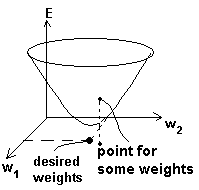
\includegraphics[width=0.40\textwidth]{error_surface.png}
\end{center}

\noindent Let $w_{ij}$ denote the weight from node $j$ in the previous layer to node $i$ in the current layer. Gradient descent updates parameters along the negative gradient:
\begin{equation}
  \Delta w_{ij} = -r\,\frac{\partial E}{\partial w_{ij}},
\end{equation}
where $r$ is the learning-rate parameter (a normalizing multiplier controlling the step size).

\subsection{Derivation of the generalized delta rule}
For a neuron $i$ in some layer,
\begin{equation}
  z_i = \sum_j w_{ij} a_j + b_i,
  \qquad a_i = g(z_i),
\end{equation}
where $a_j$ are activations from the previous layer. By the chain rule,
\begin{equation}
  \frac{\partial E}{\partial w_{ij}}
  = \frac{\partial E}{\partial a_i}\,
    \frac{\partial a_i}{\partial z_i}\,
    \frac{\partial z_i}{\partial w_{ij}}
  = \frac{\partial E}{\partial a_i}\, g'(z_i)\, a_j.
\end{equation}
Hence,
\begin{equation}\label{eq:weight_update_component}
  \Delta w_{ij}
  = -r\left(\frac{\partial E}{\partial a_i}\right) g'(z_i)\, a_j.
\end{equation}

\paragraph{Output layer.}
For an output unit $i$,
\begin{equation}
  \frac{\partial E}{\partial a_i}
  = \frac{\partial}{\partial a_i}\left(\frac{1}{2}(d_i-a_i)^2\right)
  = -(d_i-a_i).
\end{equation}
Substituting into \eqref{eq:weight_update_component} yields
\begin{equation}
  \Delta w_{ij} = r\, a_j\,(d_i-a_i)\, g'(z_i).
\end{equation}

\paragraph{Hidden layers.}
For a hidden unit $i$, the error depends on $a_i$ only through units $k$ in the next layer. Using the chain rule,
\begin{equation}
  \frac{\partial E}{\partial a_i}
  = \sum_k \frac{\partial E}{\partial z_k}\frac{\partial z_k}{\partial a_i}
  = \sum_k \frac{\partial E}{\partial z_k}\, w_{k i},
\end{equation}
since $z_k = \sum_j w_{k j} a_j + b_k$ implies $\partial z_k/\partial a_i = w_{k i}$.

\subsection{Local error signal (delta / beta)}
Define the local error signal (often called \emph{delta}; here denoted $\beta$) by
\begin{equation}
  \beta_i \stackrel{\mathrm{def}}{=} (d_i-a_i)\,g'(z_i)
  \qquad\text{(output units)}.
\end{equation}
For hidden units,
\begin{equation}
  \beta_i = g'(z_i)\sum_k w_{k i}\,\beta_k.
\end{equation}
With this notation the update is local:
\begin{equation}
  \Delta w_{ij} = r\, a_j\, \beta_i.
\end{equation}

\subsection{Sigmoid-specific form}
When the activation is the sigmoid $g(z) = 1/(1+e^{-z})$, the derivative simplifies in terms of the activation itself:
\begin{equation}
  g'(z_i) = \frac{1}{1+e^{-z_i}} \cdot \frac{e^{-z_i}}{1+e^{-z_i}} = a_i(1-a_i),
\end{equation}
so the recursive formulas reduce to
\begin{align}
  \Delta w_{ij} &= r\, a_i\, a_j\, (1-a_i)\, \beta_i,\\
  \beta_i &= (d_i - a_i)\, a_i\, (1-a_i) && \text{(output units)},\\
  \beta_i &= a_i\, (1-a_i)\, \sum_k w_{ki}\, \beta_k && \text{(hidden units)}.
\end{align}
These three equations appear constantly in the neural-network literature of this period.

\subsection{Tensor (matrix) form}
Let $a$ be the vector of activations from the previous layer and $\beta$ the vector of local error signals in the current layer. The component-wise rule $\Delta w_{ij}=r\,a_j\,\beta_i$ is the outer product
\begin{equation}
  \Delta W = r\,\beta\,a^\top.
\end{equation}

\subsection{Backpropagation algorithm (outline)}
\begin{algorithm}[H]
\caption{Backpropagation training for a feed-forward network}
\begin{algorithmic}[1]
\STATE Choose a learning rate $r$ and initialize weights/biases (small random values).
\REPEAT
\FOR{each training example $(x,d)$}
  \STATE \textbf{Forward pass:} compute activations layer by layer.
  \STATE \textbf{Compute output error:} $\beta^{(L)} = (d-a^{(L)})\odot g'(z^{(L)})$.
  \STATE \textbf{Backward pass:} for $\ell=L-1,\dots,1$ compute
         $\beta^{(\ell)} = g'(z^{(\ell)})\odot\left(W^{(\ell+1)}\right)^\top \beta^{(\ell+1)}$.
  \STATE \textbf{Update:} $W^{(\ell)} \leftarrow W^{(\ell)} + r\, \beta^{(\ell)}(a^{(\ell-1)})^\top$
         (and similarly for biases).
\ENDFOR
\UNTIL{a stopping criterion is met (error threshold, maximum epochs, or validation performance).}
\end{algorithmic}
\end{algorithm}

\subsection{Learning rate and momentum}
The learning rate $r$ should be chosen as large as possible without driving the training into oscillation. A rate that is too small makes learning unbearably slow; a rate that is too large causes the error to oscillate or diverge and learning stops altogether. To stabilize the update without sacrificing speed, the weight change is often made dependent on the previous weight change via a \emph{momentum} term:
\begin{equation}
  \Delta w_{ij}(t+1) = r\, \beta_i\, a_j + \alpha\, \Delta w_{ij}(t),
\end{equation}
where $\alpha \in [0,1)$ is the momentum coefficient. Training with a constant $r$ alone is usually a tedious trial-and-error process.

\begin{center}
  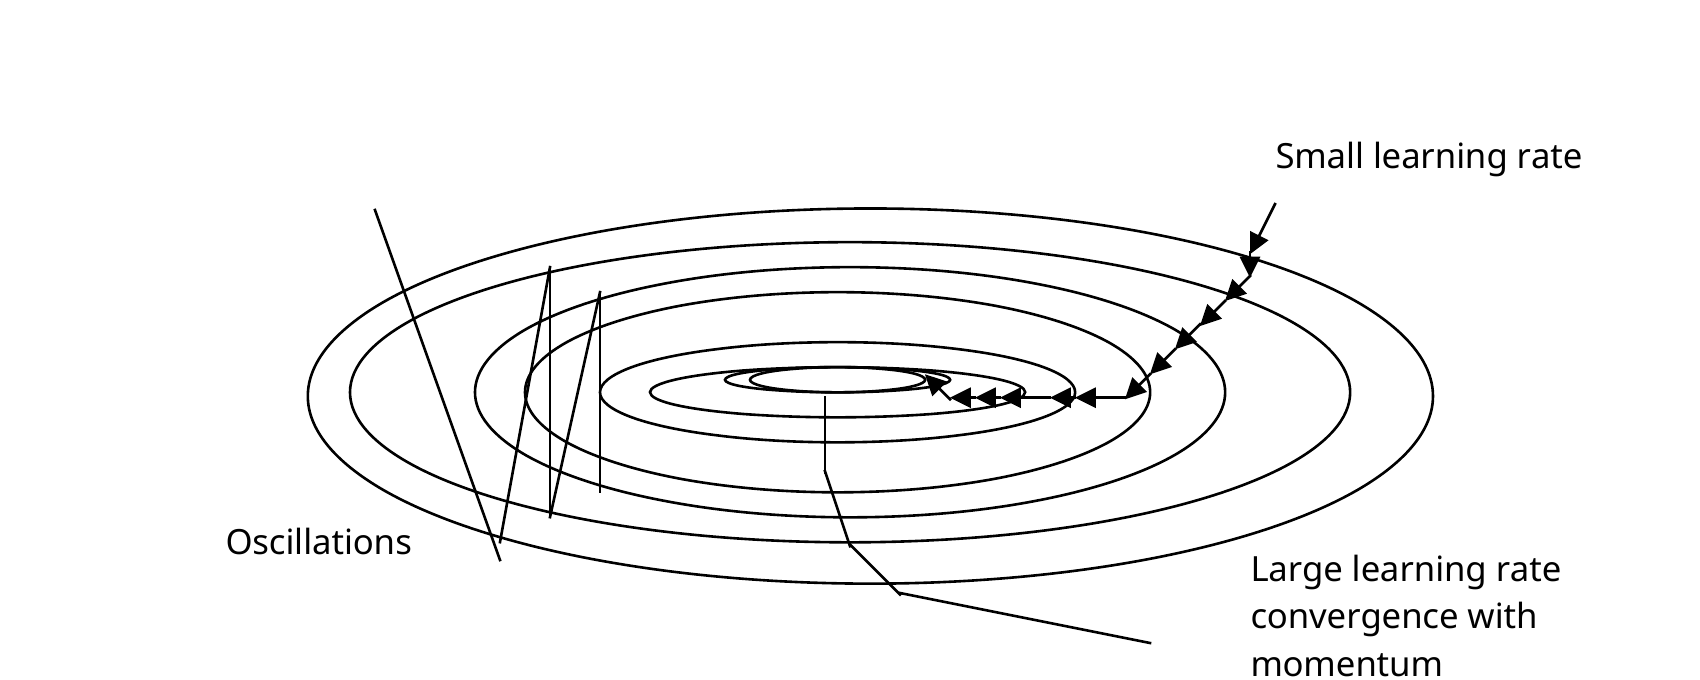
\includegraphics[width=0.7\textwidth]{learning_rate_paths.png}
\end{center}
\begin{center}
\small Convergence paths on a quadratic error surface (contour lines shown) for three learning-rate regimes: a small $r$ inches along the gradient, a too-large $r$ oscillates across the valley, and a large $r$ combined with momentum cuts the fastest path to the minimum.
\end{center}

Standard backpropagation can be slow, especially with a fixed learning rate. Many modifications have been proposed to speed convergence, including Quickprop and RPROP. \editornote{Modern practice has converged on the Adam optimizer family (Kingma \& Ba, 2014) and SGD with momentum, combined with explicit learning-rate schedules (warmup, cosine decay, step decay). Fixed learning rates are now rare outside of toy examples. Quickprop and RPROP are mostly of historical interest.}

\section{Applications}
Pattern recognition is one of the most elaborated and successful domains for neural networks. Speech recognition, text and character recognition, handwriting recognition, vision tasks, and classification of radar/sonar signals are all examples. Marketing planning, stock-market prediction, and robotics sensing can also be formulated as pattern-recognition problems. Pattern classification can be viewed as a function mapping a domain of images (or feature vectors) to a finite set of output categories.

\begin{center}
  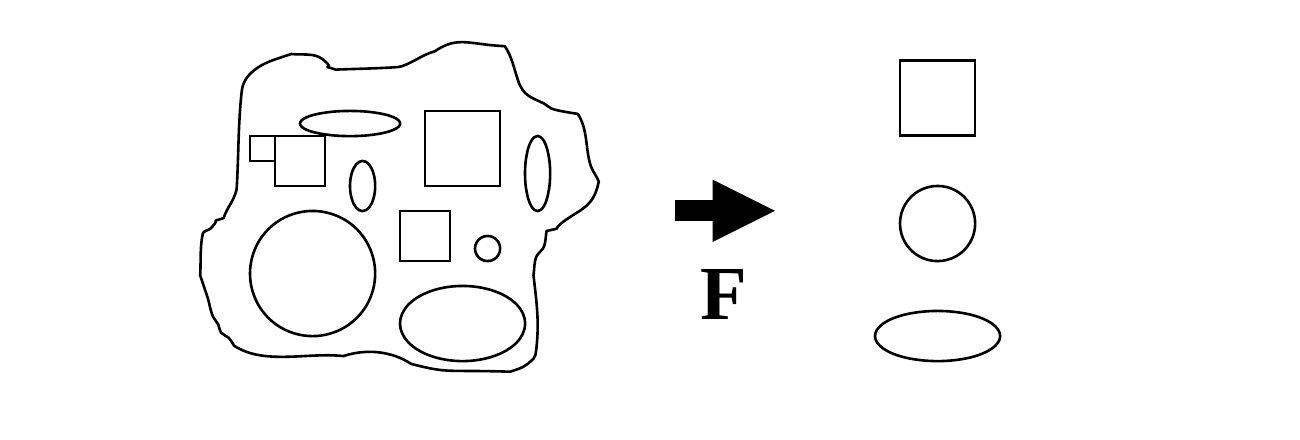
\includegraphics[width=0.65\textwidth]{pattern_classification.png}
\end{center}
\begin{center}
\small Pattern classification as a function $F$: an input image of mixed shapes is mapped to one of a finite set of output categories: here three (square, circle, ellipse).
\end{center}

Two concrete applications are described below: (i) classifying cells for cancer diagnosis and (ii) handwritten digit recognition. In both cases, the systems use backpropagation-trained feed-forward networks.

\subsection{Classifying cells for cancer diagnosis}
\emph{Source:} Ciamac Moallemi (see Bibliography).

The goal of this work is to reduce routine manual microscopy by classifying cell images into ``well'' (useful) versus ``not well'' categories for cancer diagnosis. A key requirement is high recall of well cells: if a well cell is classified as not well, potentially valuable diagnostic information may be lost.

\subsubsection{Data and processing pipeline}
Images of size $256\times 240$ pixels with 256 gray levels were used. Processing is divided into four steps:
\begin{enumerate}[leftmargin=1.2em]
  \item thresholding,
  \item segmentation,
  \item feature extraction,
  \item classification (performed by the neural network).
\end{enumerate}

\paragraph{1) Thresholding.}
The goal is to separate objects from background. The image is partitioned into 16 equal segments (approximately $32\times 120$ pixels each) in order to make the background more homogeneous within each segment. Background is then removed from each segment separately. Significant discontinuities in each histogram are removed, and the system selects an intensity threshold for the background. Pixels with gray-level values above this threshold are treated as background and assigned white.

\begin{center}
  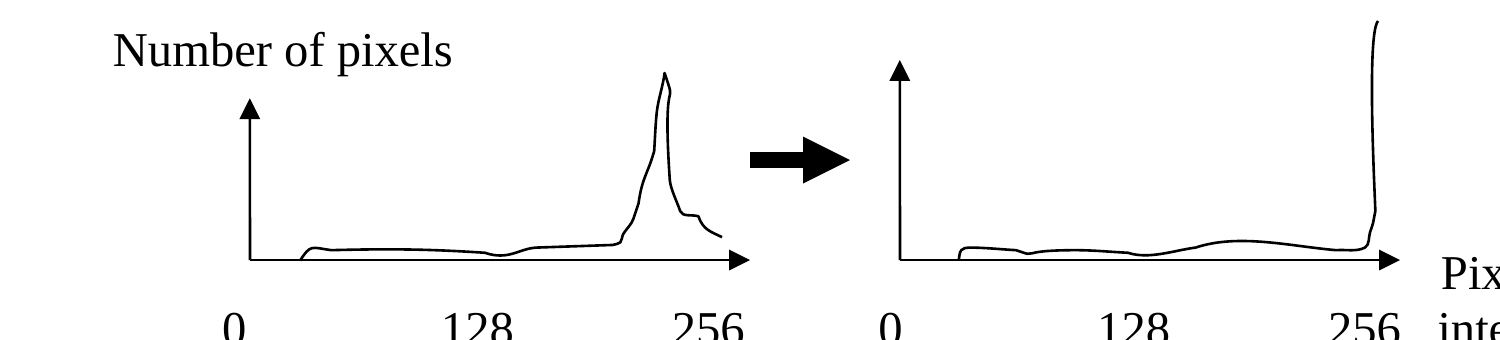
\includegraphics[width=0.7\textwidth]{thresholding_histograms.png}
\end{center}
\begin{center}
\small Pixel-intensity histogram before and after thresholding. The background peak (left) collapses onto the white bin (right), leaving the foreground pixels separated from background.
\end{center}

\paragraph{2) Segmentation.}
Objects are separated using a ``blob coloring'' algorithm (see Ballard \& Brown). The algorithm sweeps an L-shaped template across the image and assigns a distinct color to each connected object. The method can be stated as:

\begin{center}
  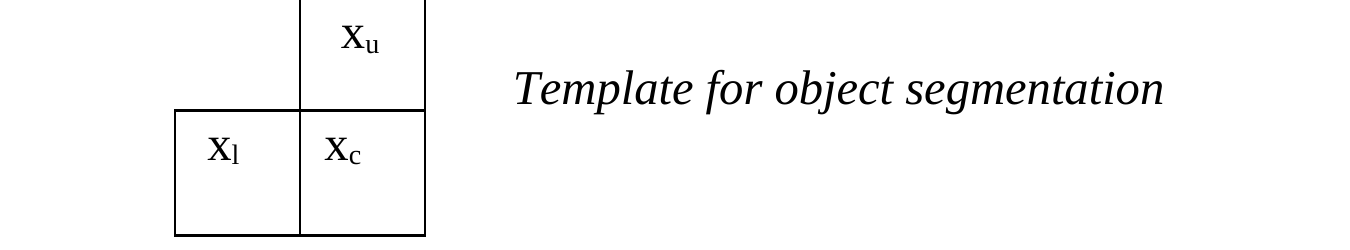
\includegraphics[width=0.32\textwidth]{segmentation_template.png}
\end{center}
\begin{center}
\small L-shaped three-pixel template used by the scan: $x_c$ is the current pixel, $x_u$ its upper neighbor, and $x_l$ its left neighbor.
\end{center}

\begin{algorithm}[H]
\caption{Blob-coloring segmentation (outline)}
\begin{algorithmic}[1]
\STATE Let the color counter $k \leftarrow 1$.
\STATE Define $f(x)=0$ if $x$ is a background pixel, and $f(x)=1$ otherwise.
\WHILE{there remain unprocessed pixels}
  \STATE Scan the image from top to bottom and left to right until $f(x_c)=1$.
  \IF{$f(x_u)=1$ and $f(x_l)=0$} \STATE $color(x_c)\leftarrow color(x_u)$ \ENDIF
  \IF{$f(x_l)=1$ and $f(x_u)=0$} \STATE $color(x_c)\leftarrow color(x_l)$ \ENDIF
  \IF{$f(x_l)=1$ and $f(x_u)=1$}
     \STATE Merge labels: $color(x_u)\leftarrow color(x_c)$ and $color(x_l)\leftarrow color(x_c)$
  \ENDIF
  \IF{$f(x_l)=0$ and $f(x_u)=0$}
     \STATE $color(x_c)\leftarrow k$; $k\leftarrow k+1$
  \ENDIF
\ENDWHILE
\end{algorithmic}
\end{algorithm}

\begin{center}
  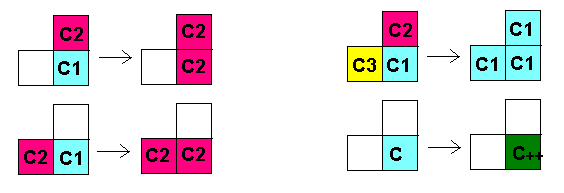
\includegraphics[width=0.75\textwidth]{meta_image_1.png}
\end{center}
\begin{center}
\small Blob-coloring transitions: assigning, propagating, merging, and starting a new label.
\end{center}

After this step, objects larger than 20 pixels can be detected reliably by their assigned labels.

\paragraph{3) Feature extraction.}
Features are numerical descriptors of each segmented object. Five features are used:
\begin{enumerate}[leftmargin=1.2em]
  \item object area (typically 100--400 pixels),
  \item circularity (ratio of object area to enclosing rectangle; typically 0.6--0.85),
  \item nuclear area (nucleus segmented by thresholding with constant 0.9; typically $<150$ pixels but $>20$),
  \item nuclear circularity (typically above 0.35),
  \item ratio of nuclear area to total cell area (typically below 0.85).
\end{enumerate}

\paragraph{4) Classification by neural network.}
The extracted features form the neural-network input. The fully connected network has 5 input nodes, two hidden layers of 10 nodes each, and 1 output node. An output value greater than 0.5 signifies a ``well'' cell.

\begin{center}
  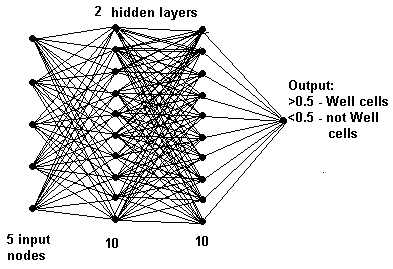
\includegraphics[width=0.55\textwidth]{meta_image_2.png}
\end{center}
\begin{center}
\small Cancer-cell classifier: 5 inputs $\to$ 10 $\to$ 10 $\to$ 1 output; $>0.5$ signifies a well cell.
\end{center}

The architecture was selected experimentally: smaller networks did not adapt well to the training set, while larger networks trained too slowly and generalized poorly. Training used Quickprop (a variant of backpropagation). Quickprop updates each weight using the gradient at two consecutive steps:
\begin{equation}
  \Delta w(t) = \frac{\partial E / \partial w (t)}{\partial E / \partial w(t-1) \;-\; \partial E / \partial w(t)} \cdot \Delta w(t-1).
\end{equation}

\subsubsection{Results}
A previously developed ``selective mapping'' algorithm based on a tree classifier achieved a misclassification level of 23.1\%, which is not acceptable for clinical use. The neural-network classifier reduced the error rates to 6.4\% for well cells and 3\% for not-well cells, with an overall error rate of 3.5\%. Computation was fast: approximately three seconds per image on a Sun 3/80, benefiting from the parallel structure of the computations.

\subsection{Handwritten digit recognition using constrained automatic learning}
\emph{Source:} LeCun et al.\ (see Bibliography).

This work addressed recognition of handwritten zip codes on postal envelopes. Digits may be incomplete, blotchy, or of poor quality. Classical pixel-based classifiers often perform poorly because they do not incorporate prior knowledge about the problem. Experiments showed that a large unconstrained network can be difficult to train on real databases with good generalization. Performance improved when domain knowledge was incorporated into the network design.

\subsubsection{Preprocessing}
Preprocessing consisted primarily of normalizing digit shape and skew so that inputs fit within a $32\times 32$ or $16\times 16$ pixel window.

\subsubsection{Shared weights and feature maps}
A key idea is to incorporate the two-dimensional geometric nature of images and to build shift invariance into the classifier. Shared weights in early layers greatly reduce the number of free parameters and improve generalization. The network implements \emph{feature maps}: within each map, all neurons apply the same weights to different spatial locations in the input. Thus, all units in a map detect the same feature at different locations, providing translation (shift) invariance. A standard fully connected network, in contrast, would treat a translated digit as a completely new pattern.

Connections therefore act as feature detectors. The first hidden layer can detect multiple distinct local features, each of which can occur at different locations.

\begin{center}
  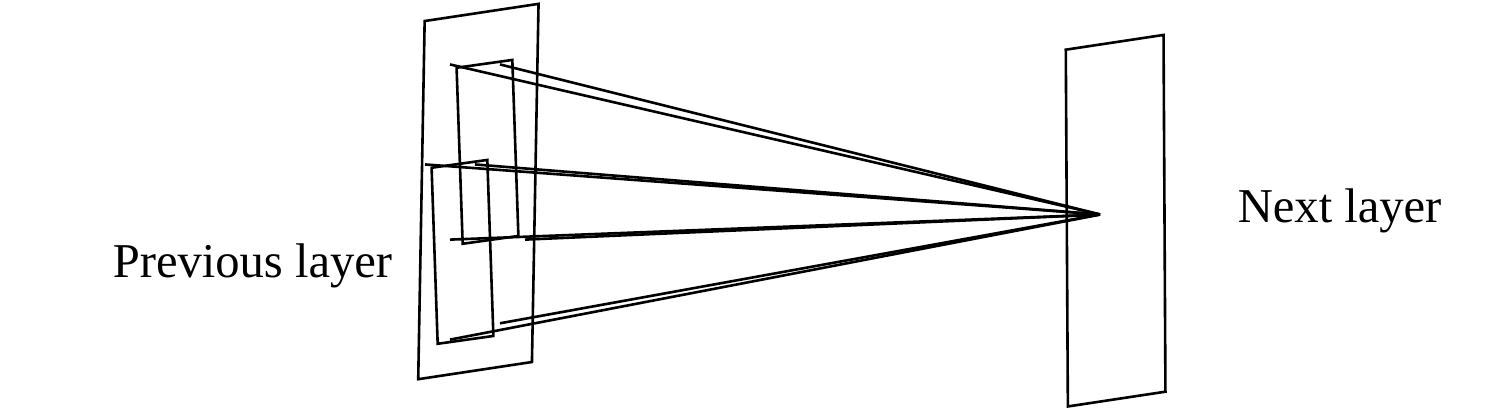
\includegraphics[width=0.7\textwidth]{feature_detector_field.png}
\end{center}
\begin{center}
\small Receptive-field connection between layers: a single unit in the next layer receives inputs only from a local patch of the previous layer. Within a feature map the same weights are reused at every patch position, so the same detector applies at every location in the input.
\end{center}

\subsubsection{Network architecture and training}
\begin{center}
  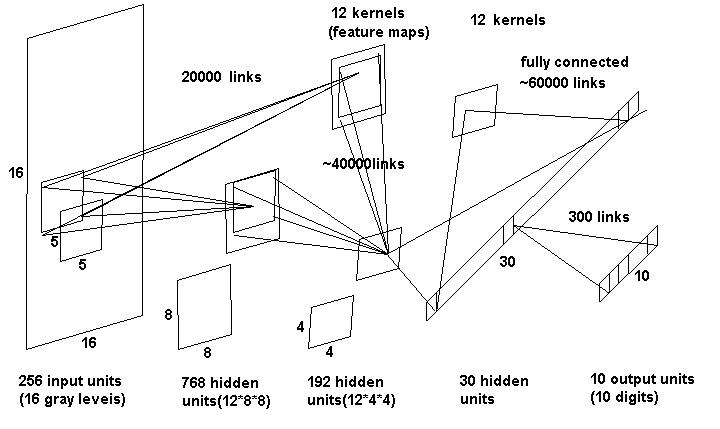
\includegraphics[width=0.85\textwidth]{meta_image_4.png}
\end{center}
\begin{center}
\small LeCun network: 256 input units (16$\times$16) $\to$ 768 hidden units (12 feature maps of 8$\times$8) $\to$ 192 hidden units (12 maps of 4$\times$4) $\to$ 30 hidden units $\to$ 10 output units. The first two hidden layers perform convolutions with shared weights; the last two are fully connected.
\end{center}

Connections within a given feature map are constrained to share weights. For example, all 64 units in a kernel (feature map) in the first hidden layer use the same set of 25 weights. Because of weight sharing, the network has 9{,}760 weights, substantially fewer than the number of potential links. The first two hidden layers perform convolutions, while the third and fourth (output) layers are fully connected and perform the final classification. \editornote{This shared-weight feature-map design is now recognized as the origin of the convolutional neural network (CNN) family that dominated image recognition from AlexNet (2012) onward.}

Weights were initialized randomly in the range $\left[-2.4/f_i,\; 2.4/f_i\right]$, where $f_i$ is the number of inputs (fan-in) to the unit associated with the connection. Mean squared error was used as the cost function. \editornote{Modern classification networks use cross-entropy loss (with a softmax output layer) rather than MSE. Cross-entropy gives stronger gradients when the prediction is far from the target, so training converges faster and more reliably. MSE is still the standard choice for regression problems.} Training was performed in an on-line (stochastic gradient) fashion: patterns were presented in a constant order for 28 passes, and weights were updated after each individual pattern. This procedure often converges faster on highly redundant data. The network was trained on 7{,}300 examples and tested on a separate set of 2{,}000 examples. The learning rate was fixed throughout training.

\subsubsection{Performance and impact}
Performance reached approximately 99\%, and the system was implemented in custom VLSI for high-speed postal sorting, achieving throughput from camera to classified digit of more than 10 digits per second. This work was among the first to demonstrate that a general-purpose neural-network chip could serve as an accelerator in a larger system, enabling real problems with strong regularities to be solved effectively by neural networks.

\begin{center}
  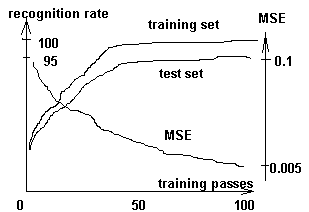
\includegraphics[width=0.45\textwidth]{meta_image_5.png}
\end{center}
\begin{center}
\small Approximate behavior of mean squared error (and recognition rate) as a function of passes through the training set.
\end{center}

\section{Summary}
Neural networks are useful when either no explicit algorithm is known for a problem, or the number of interacting variables makes hand-crafted rules impractical. Traditional application fields include pattern recognition (including signature analysis as a sub-field), speech and vision recognition, sound and vibration analysis, process control, marketing planning, stock-market prediction, and robotics / sensing.

Feed-forward networks form roughly \textbf{90\% of successful neural-network applications} (as of 1997). \editornote{This share was accurate in 1997 but no longer holds. The post-2012 deep-learning era is dominated by convolutional networks for vision, recurrent and transformer networks for sequences and language, and large generative models. Pure feed-forward networks remain the foundational building block (every modern architecture composes from them), but they are no longer the dominant deployed form.} With enough resources and training data, almost any function can be approximated to arbitrary precision by a sufficiently large feed-forward network. Backpropagation is by far the most common training method for these networks; it is slow in a naive implementation, and many variants (Quickprop, RPROP, momentum, jittering, early stopping) have been proposed to speed convergence or to escape local minima.

When a network has too many trainable weights it may become erratic and unreliable due to overfitting; a practical rule of thumb is that the number of trainable weights influencing any output should be smaller than the number of training samples. At the same time, an overly small network cannot learn the required mapping. Tuning the learning rate further complicates the trade-off.

\textbf{The single most effective lever is heuristics: incorporating problem-specific knowledge into the network design.} Two illustrations from the applications:
\begin{itemize}[leftmargin=1.2em]
  \item Two-dimensional geometry and shift invariance built into the topology of the LeCun handwritten-digit network.
  \item Sequential hidden layers performing feature extraction at successive abstraction levels, as in both applications above.
\end{itemize}

Without such heuristics, even a correctly-trained network often fails to generalize. The thesis of this report is that the architecture and preprocessing pipeline carry as much of the work as the gradient-descent algorithm itself; they are necessary, not cosmetic.

\section{Bibliography}
\begin{enumerate}[leftmargin=1.2em]
  \item D.\ E.\ Rumelhart, G.\ E.\ Hinton, and R.\ J.\ Williams, ``Learning representations by back-propagating errors,'' \emph{Nature}, 323(6088), October 1986, pp.\ 533--536.
  \item Ben J.\ A.\ Kr\"{o}se and Patrick van der Smagt, \emph{An Introduction to Neural Networks}, 4th edition, September 1991.
  \item Stuart Russell and Peter Norvig, \emph{Artificial Intelligence: A Modern Approach}, Prentice Hall, 1995, pp.\ 563--591.
  \item Y.\ LeCun et al., ``Handwritten Digit Recognition: Applications of Neural Network Chips and Automatic Learning,'' \emph{IEEE Communications Magazine}, November 1989, 27(11), pp.\ 41--46.
  \item Ciamac Moallemi, ``Classifying Cells for Cancer Diagnosis Using Neural Networks,'' \emph{IEEE Expert}, December 1991, pp.\ 8--12.
  \item G.\ Dreyfus, ``Neural Networks for Automatic Recognition of Handwritten Digits,'' in \emph{Applications of Neural Networks}, edited by H.\ G.\ Schuster, VCH.
  \item D.\ H.\ Ballard and C.\ M.\ Brown, \emph{Computer Vision}, Prentice Hall, Englewood Cliffs, NJ, 1982.
  \item Online resources (as originally consulted):\\
  \url{ftp://ftp.sas.com/pub/neural/}\\
  \url{http://www.shef.ac.uk/psychology/gurney/notes/contents.html}\\
  \url{http://www.cs.stir.ac.uk/~lss/NNIntro/InvSlides.html}\\
  \url{http://www.mcs.com/~drt/bprefs.html}
\end{enumerate}

\end{document}
